% 页面设置
\documentclass[12pt, a4paper]{article} % 字号:12,纸张:A4
\usepackage[top=2.54cm, bottom=2.54cm, left=3.18cm,right=3.18cm]{geometry} % 页边距设置
% 字体设置
\usepackage[UTF8]{ctex}
\usepackage{fontspec} % 设置字体
%\setCJKmainfont{SimSun}[AutoFakeBold=true, BoldFont={SimHei}, ItalicFont={KaiTi}] % 正文字体
%\setCJKsansfont[AutoFakeBold=3]{KaiTi} % 无衬线字体
%\setCJKmonofont[AutoFakeBold=3]{SimHei} % 等宽字体
\setmainfont{Times New Roman} % 设置主字体为新罗马体
% 文本设置
\usepackage{enumerate} % 支持小标题编号
\linespread{1.5} % 行间距1.5倍
\usepackage{indentfirst}%首段缩进
\setlength{\parindent}{2em} % 首行缩进两字符
\usepackage[hidelinks]{hyperref} % 目录添加超链接
\usepackage{zhnumber} % 章节标题中文显示
\usepackage[cmyk]{xcolor} % 文字彩色显示
% 数学支持
\usepackage{amsmath} % 数学公式支持
\usepackage{amssymb} % 数学符号支持
\usepackage{bm} % 公式加粗
\usepackage{mathrsfs} % 花体字母
\usepackage{yhmath} % 更多的数学符号
% 图片设置
\usepackage{caption} % 插入图片标题
\usepackage{float} % 控制图片位置
\usepackage{subfigure} % 图片并排
\usepackage{booktabs} % 插入表格
% 表格设置
\usepackage{multirow} % 表格自动换行
\usepackage{bigstrut} % 表格间距
\usepackage{rotating} % 表格旋转
\usepackage{tabularx} % 表格宽度
\usepackage{colortbl} % 表格颜色
\usepackage{graphicx} % 表格自动宽度

\title{第一章 \ \ \ 绪论} % 文章标题
\author{Castor Ye} % 文章作者
\date{} % 文章时间

\begin{document} % 文档从这里开始。
\maketitle % 按照预定的模板把上面那些信息排好。
\newtheorem{definition}{定义}[section]
\newtheorem{theorem}{定理}[section]
\newtheorem{example}{例}[section]
\newtheorem{solution}{题解}
\newtheorem{algorithm}{算法}
\newtheorem{axiom}{公理}
\newtheorem{property}{性质}
\newtheorem{proposition}{命题}
\newtheorem{lemma}{引理}
\newtheorem{corollary}{推论}[section]
\newtheorem{remark}{注解}
\newtheorem{condition}{条件}
\newtheorem{conclusion}{结论}
\newtheorem{assumption}{假设}
\renewcommand{\figurename}{图} % 将图片序号改为图
\renewcommand{\tablename}{表} % 将表格序号改为表
%%%%%%%%%%%%%%%%%%%%%%%%%%%%%%%%%%%%%%%%%%%%%%%%%%%%%%%%%%%%%%%%%%%%%%%
% 文章内容从此开始
\section{引言}

机器学习是这样一门学科,它致力于研究如何通过计算的手段,利用经验来改善系统自身的性能。在计算机系统中,“经验”通常以“数据”的形式存在,因此,机器学习所研究的主要内容,是关于在计算机上从数据中产生“模型”(model)的算法,即“学习算法”(learning algorithm)。

有了学习算法,我们吧经验数据提供给它,它就能基于这些数据产生模型;在面对新的情况时,模型会给我们提供相应的判断。

\section{基本术语}

要进行机器学习,先要有数据。假定我们收集了一批关于西瓜的数据,例如:(色泽=青绿;根蒂=蜷缩;敲声=浊响),(色泽=乌黑;根蒂=蜷缩;敲声=清脆)等等,每对括号内是一条记录。

这组记录的集合称为一个“数据集”(data set),其中每条记录是关于一个事件或对象(这里为一个西瓜)的描述,称为一个“示例”(instance)或“样本”(sample)。反映事件或对象在某方面的表现或性质的事项,例如“色泽”“根蒂”等,称为“属性”(attribute)或“特征”(feature);属性上的取值,例如“青绿”,“乌黑”等,称为“属性值”(attribute value)。属性张成的空间称为“属性空间”(attribute space)、“样本空间”(sample space)或“输入空间”。

例如,我们把“色泽”“根蒂”“敲声”作为三个坐标轴,则它们张成一个用于描述西瓜的三维空间,每个西瓜都可以在这个空间中找到自己的坐标位置。由于空间中的每个点对应一个坐标向量,因此我们也把一个示例称为一个“特征向量”(feature vector)。

一般地,令 $D = \{x_1, x_2, \cdots, x_m\}$ 表示包含 $m$ 个示例的数据集,每个示例由 $d$ 个属性描述,则每个示例 $x_i = (x_{i1}, x_{i2}, \cdots, x_{id})$ 是 $d$ 维样本空间 $\chi$ 中的一个向量,$x_i \in \chi$,其中 $x_{ij}$ 是 $x_i$ 在第 $j$ 个属性上的取值,$d$ 称为样本 $x_i$ 的“维数”(dimensionality)。

从数据中学得模型的过程称为“学习”(learning)或“训练”(training),这个过程通过执行某个学习算法来完成。训练过程中使用的数据称为“训练数据”(train data),其中每个样本称为一个“训练样本”(training sample),训练样本组成的集合称为“训练集”(training set)。学得模型对应了关于数据的某种潜在的规律,因此亦称“假设”(bypothesis);这种潜在规律自身,则称为“真相”或“真实”(ground-truth),学习的过程就是为了找出或逼近真相。

关于示例结果的信息,例如“好瓜”,称为“标记”(label);拥有了标记信息的示例,则称为样例(example)。一般地,用 $(x_i, y_i)$ 表示第 $i$ 个样例,其中 $y_i \in Y$ 是示例 $x_i$ 的标记,$Y$ 是所有标记的集合,亦称“标记空间”(label space)或“输出空间”。

若我们预测的是离散值,例如“好瓜”“坏瓜”,此类学习任务称为“分类”(classification);若欲预测的是连续值,例如西瓜的成熟度0.95、0.92,此类学习任务称为“回归”(regression)。对只涉及两个类别的“二分类”(binary classification),通常称其中一个为“正类”(positive class),另一个类为“反类”(negative class);涉及多个类别时,则称为“多分类”(multi-class classification)任务。

学得模型后,使用其进行预测的过程称为“测试”(testing),被预测的样本称为“测试样本”(testing sample)。

我们还可以对西瓜做“聚类”(clustering),即将训练集中的膝盖分成若干组,每组称为一个“簇”(cluster)。

根据训练数据是否拥有标记信息,学习任务可大致划分为两大类:“监督学习”(supervised learning)和“无监督学习”(unsupervised learning),分类和回归是前者的代表,而聚类则是后者的代表。

需要注意的是,机器学习的目的是使学得的模型能很好地适用于“新样本”,这种适应新样本的能力称为“泛化”(generalization)能力。假设样本空间中全体样本服从一个未知的“分布”(distribution)$D$,我们获得的每个样本都是独立地从这个分布上采样获得的,即“独立同分布”(independent and identically distribution,i.i.d)。一般而言,训练样本越多,我们得到的关于 $D$ 的信息也越多,更有可能训练出具有强泛化能力的模型。

\begin{figure}[H]
    \centering
    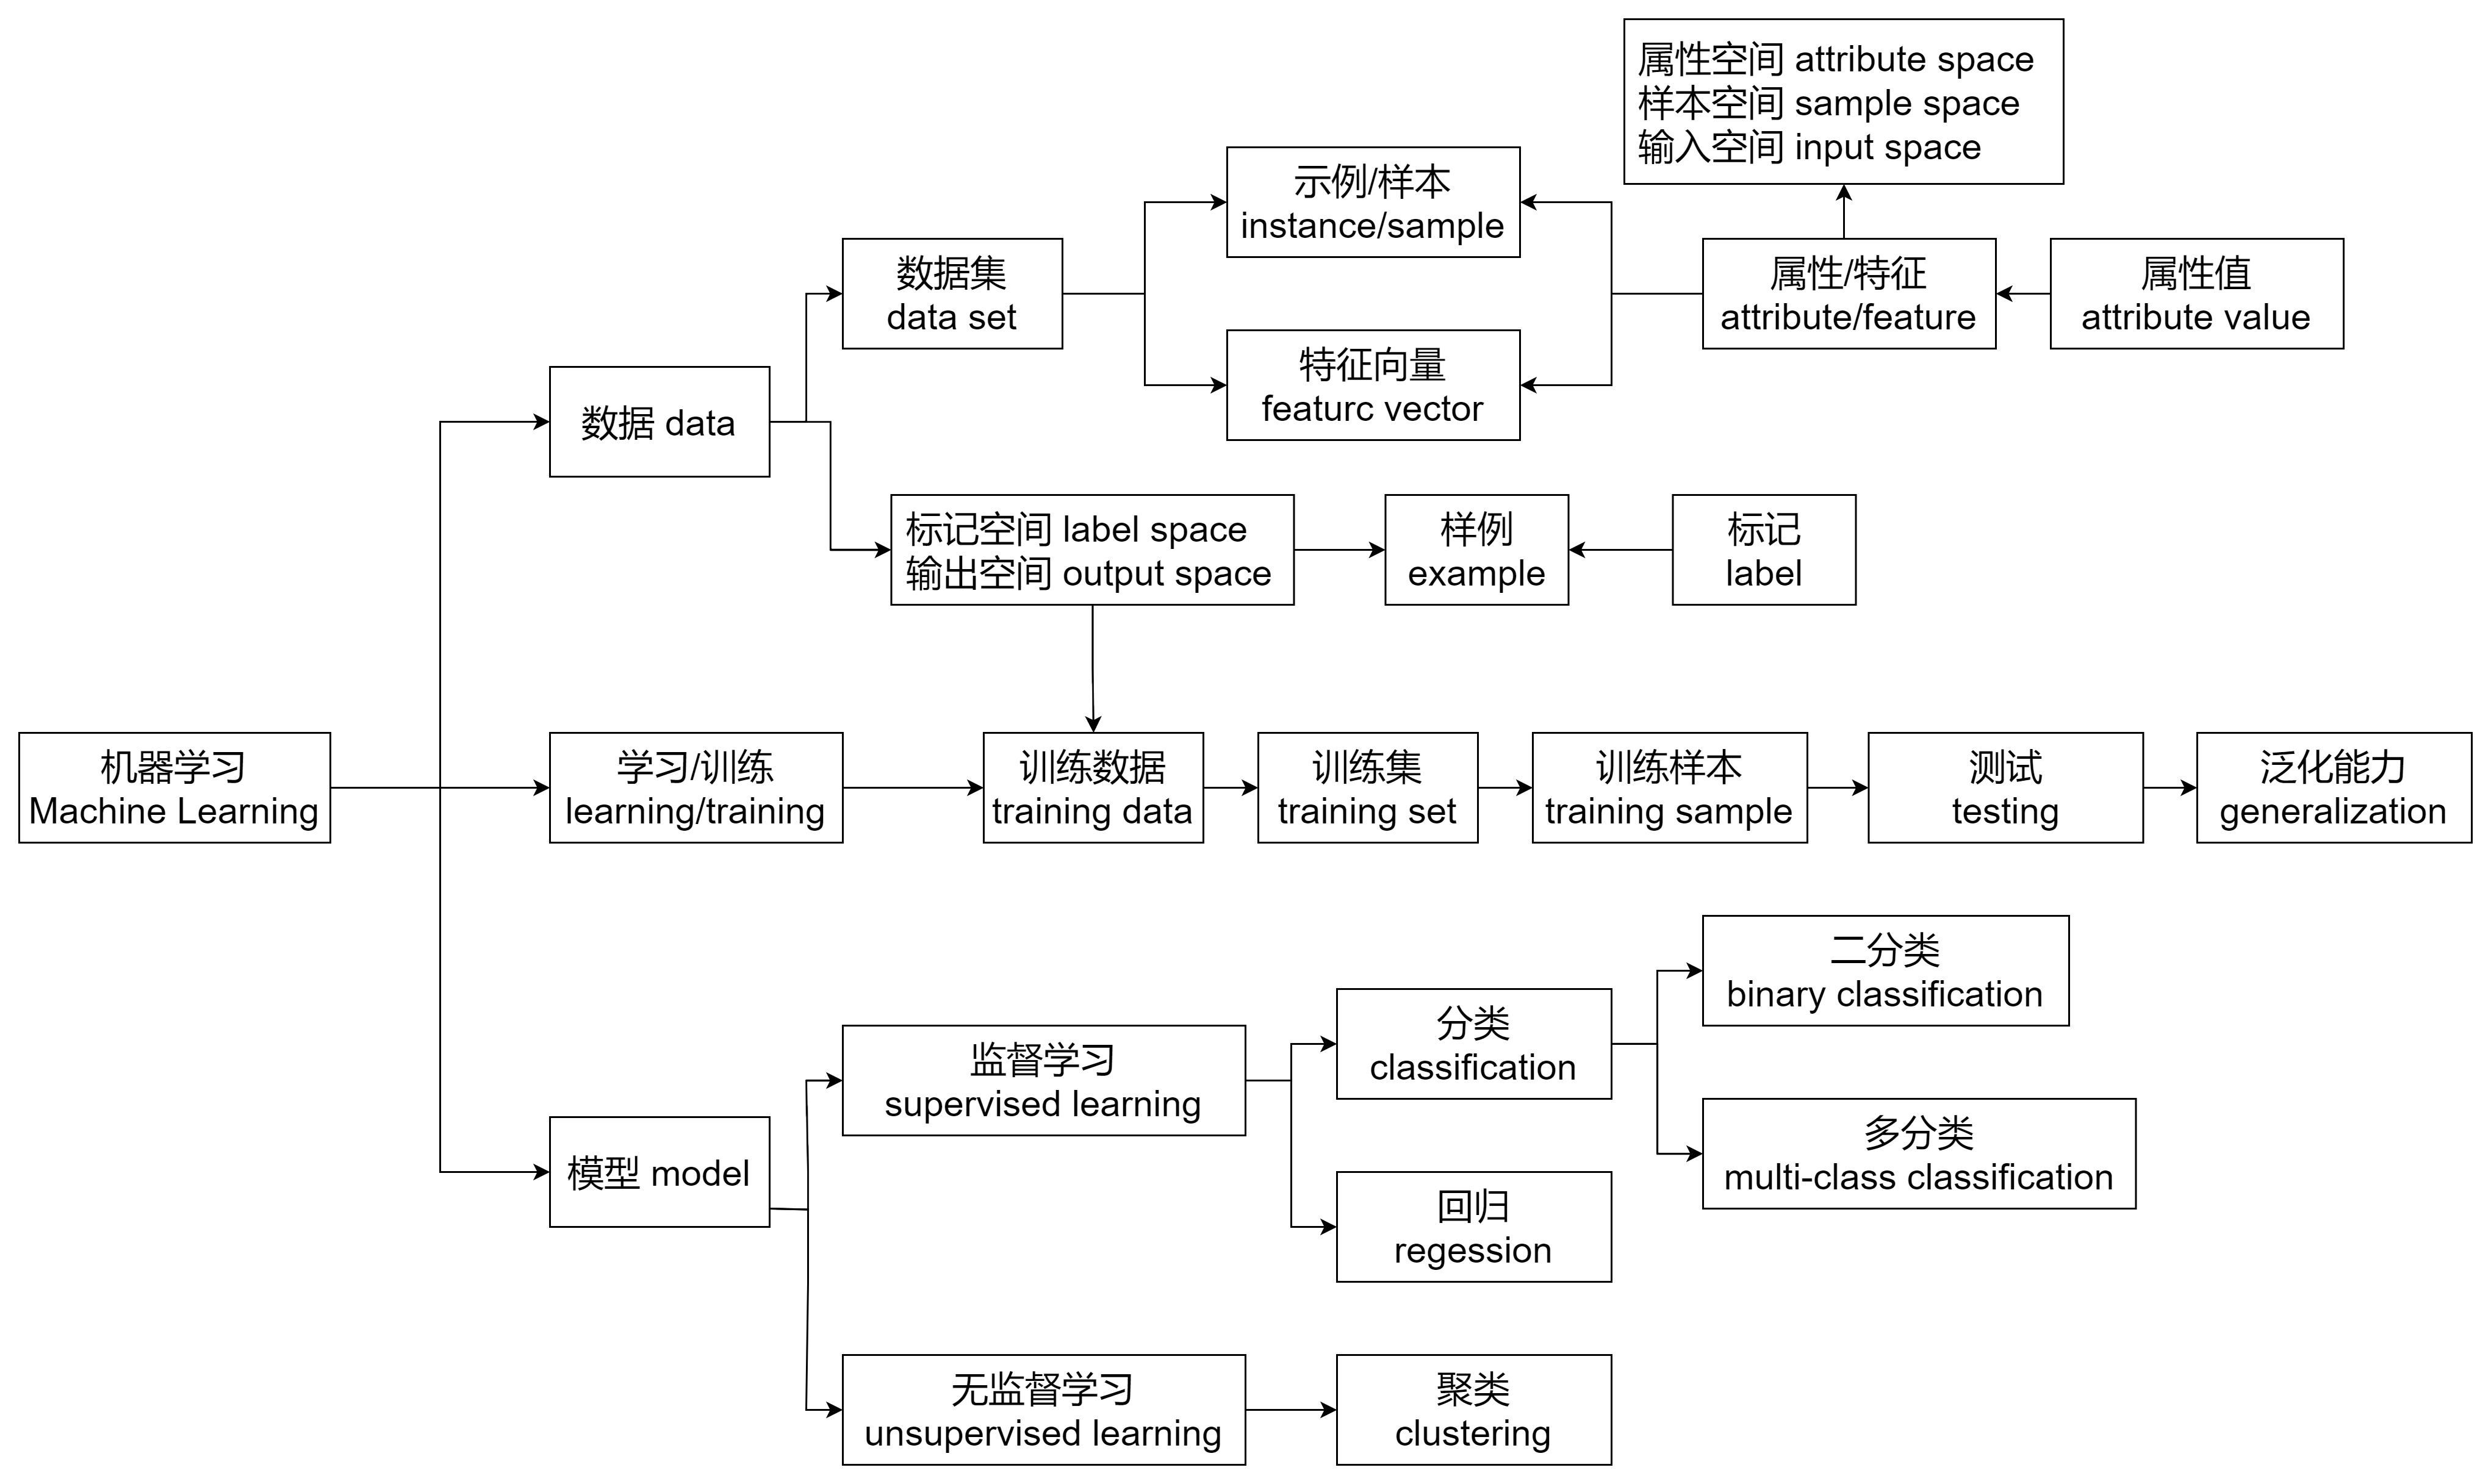
\includegraphics[width=1\textwidth]{../img/1-1-基本术语.drawio.png}
    \caption{基本术语}
    \label{fig:1-1-基本术语.drawio.png}
\end{figure}

\section{假设空间}




\end{document}